\documentclass[12pt]{beamer}



\setbeamertemplate{headline}{
\begin{beamercolorbox}[wd=\paperwidth]{chcolor}
\end{beamercolorbox}
}

%\usepackage[japanese]{babel}
\usepackage{xeCJK}
 \setCJKmainfont[BoldFont=../fonts/AozoraMincho-bold,AutoFakeSlant=0.15]{../fonts/AozoraMinchoRegular.ttf}
%\setCJKmainfont[BoldFont=NotoSansCJKjp-Bold,AutoFakeSlant=0.15]{Noto Sans CJK JP}


\usepackage[size=a0,orientation=landscape,scale=1.4]{beamerposter}
\geometry{paperwidth=1600mm,paperheight=900mm}
\usepackage{amssymb}
\usepackage{amsmath}
\usepackage{dsfont}
\usepackage{gensymb}


\setbeamerfont{title}{family=\rmfamily}
%\setbeamercolor{title}{fg=red!50!blue!30}
 \setbeamercolor{title}{fg=black}
 \setbeamercolor{frametitle}{fg=black}
%\usepackage{fontspec}
\usefonttheme{professionalfonts} % using non standard fonts for beamer
%\usefonttheme{serif} % default family is serif

\setbeamertemplate{frametitle}{\vspace{1mm}\color{black}\bfseries\large\insertframetitle\par\vskip-6pt\hrulefill\par\normalsize\insertframesubtitle}
\setbeamertemplate{footline}{\qquad\color{black}\bfseries\insertframenumber\vspace{3mm}}
%\setbeamertemplate{footline}{\vspace{5mm}}
\setbeamertemplate{itemize item}{\color{black}\tiny$\blacksquare$}
\addtobeamertemplate{footnote}{}{\vspace{-2ex}}

\newcommand\Fontvi{\fontsize{9}{7.2}\selectfont}

\usepackage{xcolor,graphicx}
\usepackage[outdir=figures/converted_figs/]{epstopdf}
\usepackage{subfig,float}
\usepackage[figurename=Fig.,tablename=Tab.]{caption}% center as possible option
\usepackage{booktabs,array,rotating,tabularx}
%\usepackage{verbatim}       %% Doesnt work with beamer

\usepackage[absolute,overlay]{textpos}
%\usepackage[texcoord,
%grid,gridcolor=red!10,subgridcolor=green!10,gridunit=pt]{eso-pic}
\setbeamerfont{footnote mark}{size=\Tiny}

\usepackage{caption}
\DeclareCaptionLabelSeparator{pipe}{ $|$ }% or $\vert$
\captionsetup{
  format=plain,
  justification=raggedright,
  singlelinecheck=false,
  font=small,
  font={bf,sf}, % This covers labelfont and textfont
  labelsep=pipe,
  figurename=Figure
}


%\captionsetup{font={tiny,onehalfspacing}}    %% messes up the footnotes

\def\eq{equation}

\usepackage{hyperref}
 \hypersetup{
    colorlinks=true,
    linkcolor=black,
    filecolor=magenta,
    urlcolor=red,
    bookmarksnumbered=true,
    citecolor=blue
 }
 \urlstyle{same}

%\usepackage[acronym,nonumberlist]{glossaries}
% \makeglossaries
% \loadglsentries{../glossary}

\usepackage{animate}
\usepackage{tikz}
 \usetikzlibrary{positioning}
 \usetikzlibrary{snakes}
%\usetikzlibrary{shapes.misc}
%\usetikzlibrary{decorations}

\newcommand{\putat}[3]{\begin{picture}(0,0)(0,0)\put(#1,#2){#3}\end{picture}}

\title{\newline\newline\newline \bfseries {Major Advanced Topics  \\ 
 \Tiny  26433101}}
\author[Fred]{\textbf{Ongonwou Fred}}
\institute{
        \textbf{Phd Candidate}\\\textbf{\hspace{2mm}2343003}
}
%\date{April 26, 2023}
\titlegraphic{
% \begin{picture}(-100,0)
%  \put(-240,167){
\includegraphics[scale=.28]{ustm_logo.png}}%\footnote{logo USTM}}
%  \put(50,155){
\includegraphics[scale=1.5]{ed-sfa_logo.jpg}}%\footnote{logo ED-SFA}}
% %\put(-150,190){\makebox(0,0)[]{\includegraphics[width=20mm]{example-image-a}}}
% \end{picture}
}




\begin{document}


\begin{frame}%[t]
\frametitle{\Huge
\begin{center}
\vspace{100pt}

Atomic, Molecular and Optical (AMO) Physics \par\vspace{50pt}
\Large
Controling matter through the help of radiation \par\vspace{30pt}
%Department of Engineering Science, The University of Electro-Communications
\end{center}
}

\framesubtitle{
\begin{center}
\small 
High harmonic generation (HHG) and photoelectron momentum distribution (PEMD) 
are some of the most 
important processes driving the study of matter-radiation interaction
and will lead to important advances in fundamental science and engineering.
Through HHG, for example, it is possible to produce coherent radiations 
outperforming the external fields in regards to frequency and pulse duration.
The current theory, valid for stationary systems, falls short at
the description of nonstationary systems, since it ignores radiations
induced by the external force. 
Following Yangaliev \textit{et al.}[1], we aim at 
extending the quantum theory of radiation for real nonstationary systems,
i.e in 3 dimensions and for realistic potentials.
\end{center}
}

% ----- First column

\begin{textblock*}{\textwidth}(100pt,600pt)
{\huge\textbf {1. Background}} \\\vspace{30pt}
%Theory and illustrations to put here

\end{textblock*}

\begin{textblock*}{1000pt}(100pt,700pt)
%\centering
%\rotatebox{90}{
  \large \textbf{Evolution of the laser field}
 \begin{minipage}{0.6\linewidth}
 \begin{figure}[tp]
 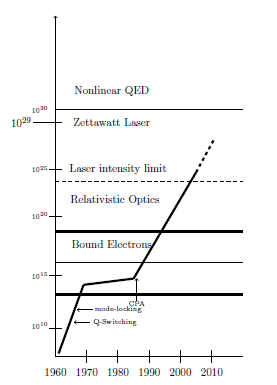
\includegraphics[scale=3., trim={0 0 0 0},clip]{images/intensity_limit.png} \\
 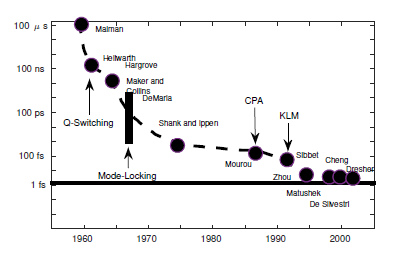
\includegraphics[scale=2., trim={0 0 0 0},clip]{images/pulse_length.png} \\
 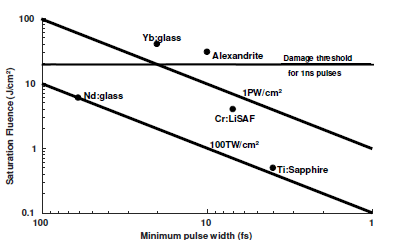
\includegraphics[scale=2., trim={0 0 0 0},clip]{images/intensity_medium.png} \\
%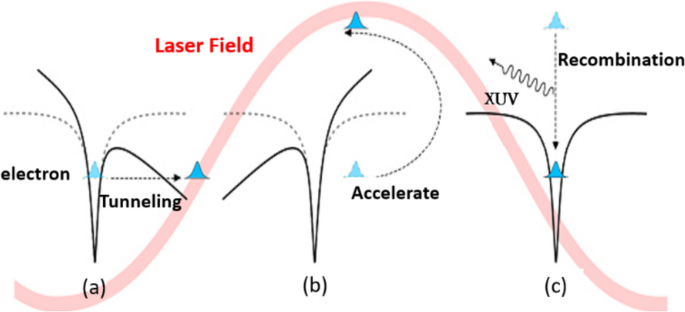
\includegraphics[scale=.50, trim={0 0 0 0},clip]{images/hhg_process.png}

%%\caption{Eigenvalues.}
%\label{fig:pemd_0114}
 \end{figure}

\end{minipage}
\end{textblock*}


\begin{textblock*}{1100pt}(800pt,700pt)
%\centering
%\rotatebox{0}{
 \begin{minipage}{0.5\linewidth}
  \ \textbf{Basic strong field phenomena} \\
 \begin{figure}[tp]
  \small 1. Multiphoton Ionization (MPI)
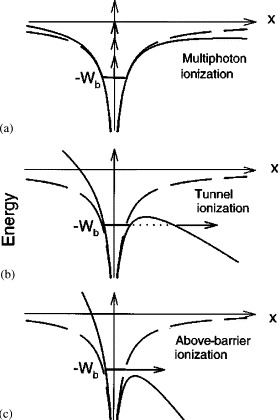
\includegraphics[scale=.9, trim={0 0 0 0},clip]{images/phenomena.png} \\
  \small 2. High harmonic generation (HHG)
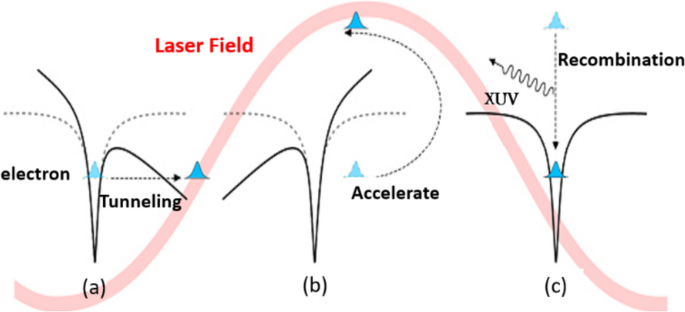
\includegraphics[scale=.7, trim={0 0 0 0},clip]{images/hhg_process.png} \\
\vspace{10pt}
 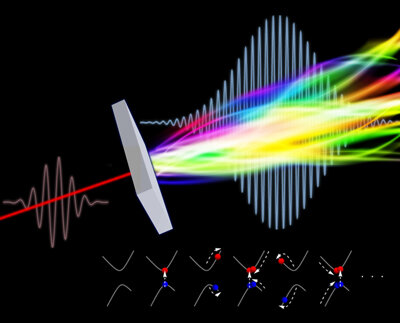
\includegraphics[scale=1., trim={0 80 0 0},clip]{images/modeling-high-harmonic.jpg} \\
  \small 3. Nonsequential double ionization (NSDI)
 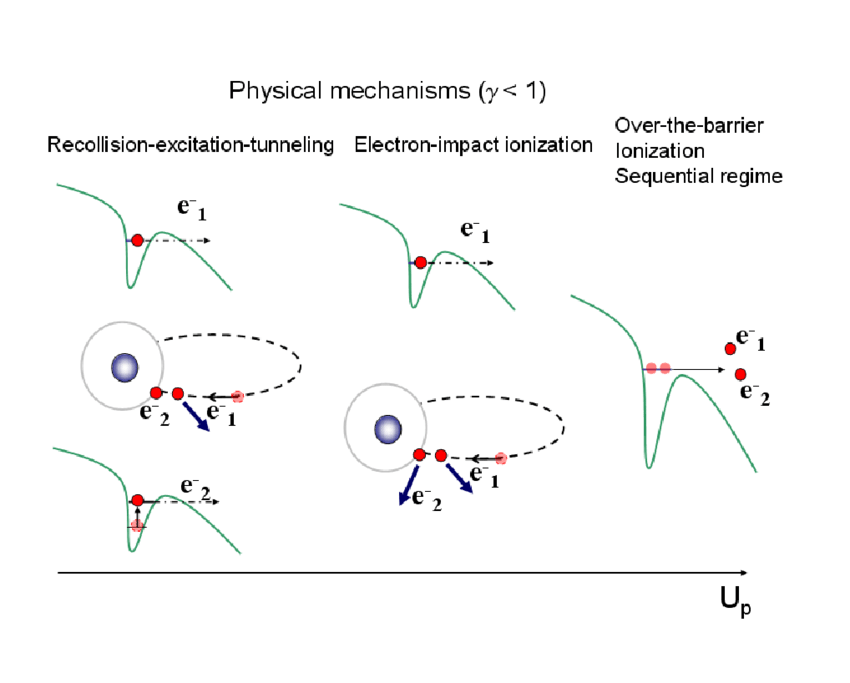
\includegraphics[scale=0.7, trim={0 20 0 0},clip]{images/nsdi_scheme.png}
 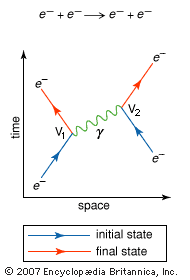
\includegraphics[scale=1.3, trim={0 0 0 10},clip]{images/nsdi_feynman.png}
%\caption{Eigenvalues.}
%\label{fig:pemd_0114}
 \end{figure}
%}
\end{minipage}
\end{textblock*}




\begin{textblock*}{0.3\textwidth}(1400pt,600pt)
{\huge\textbf {2. Theory}} \\\vspace{30pt} 
{\small \textbf{Strong field laser interaction with atoms} \\
Schr\"odinger equation
\begin{align}
 i\frac{\partial \left| \Psi(t)\right\rangle}{\partial t}
 =   \Bigg[ \hat{H}_{0} + \boldsymbol{F(t)\cdot\hat{\rm r}} \Bigg]
\left|\Psi(t)\right\rangle, \nonumber\\
 \begin{split}
 \left|\Psi(t)\right\rangle = 
  \sum_n A_n(t) e^{-iE_n t}\left| \psi_n \right\rangle  
  + \int B_{k}(t) e^{-iE_k t}\left| \psi_k^{(-)}\right\rangle dk. \nonumber
\end{split}
\end{align}
}
\vspace{20pt}

{\footnotesize
\begin{align}
\boldsymbol{F}(t) = F_0 f(t) \exp( \omega t + \varphi),
\hspace{40pt}
p(t) = - \left\langle \psi(\boldsymbol{r},t)\right| \boldsymbol{\hat{p}}
\left| \psi(\boldsymbol{r},t)\right\rangle, \nonumber
\hspace{40pt}
f(\omega) = \int e^{i\omega t} f(t) dt\hspace{30pt}\mbox{Fourier transform}
\end{align}
}


{\normalsize
{\normalsize 
\noindent Quantities relevant to the dynamics of the system are 
evaluated by exploiting the wavepacket 
$\left| \Psi(\boldsymbol{r},t)\right\rangle$}. 
The probability to find the system in any 
of the bound states $\left| \psi_n \right\rangle$ 
or excited states   $\left| \psi_k^-\right\rangle$ or excited states  
\begin{equation}
%P_n = \left| \left\langle \psi_n^-,0 |
%     \Psi(t\leqslant T)\right\rangle\right|^2,
% \hspace{10pt}
%Q_\nu = \sum_n \left| \left\langle \psi_n^-, \nu | 
%    \Psi(t\leqslant T)\right\rangle\right|^2.
%P_n = \left| A_n \right|^2,
P_n = \left| \left\langle \psi_n^-
  | \Psi(t)\right\rangle\right|^2,
 \hspace{30pt}
%Q_\nu = \sum_n \left\langle \Psi(t) | 
%  \bar{d}_\nu^\dagger \bar{d}_\nu | \Psi(t)\right\rangle|_{t\geqslant T}.
%Q(\omega) = \left| p(\omega) \right|^2.
 \nonumber
\end{equation}
}


{
\normalsize 
\noindent The survival probability and the ionization probabilities are 
\begin{equation}
P_{\rm surv} = \sum_n \left| \left\langle \psi_n
  | \Psi(t)\right\rangle\right|^2, 
 \hspace{30pt} E_n \leqslant 0, \hspace{60pt}
P_{\rm ion} = 1- P_{\rm surv}.
%Q_\nu = \sum_n \left\langle \Psi(t) | 
%  \bar{d}_\nu^\dagger \bar{d}_\nu | \Psi(t)\right\rangle|_{t\geqslant T}.
%Q(\omega) = \left| p(\omega) \right|^2.
 \nonumber
\end{equation}
\noindent and the probability density of the wavepacket is

\begin{equation}
 \mathcal{D}(\boldsymbol{r},t) = \left| \Psi(\boldsymbol{r},t)\right|^2
  =   \left| \sum_n A_n(t) e^{-iE_n t}\left| \psi_n \right\rangle  
  + \int B_{k}(t) e^{-iE_k t}\left| \psi_k^{(-)}\right\rangle dk.\right|^2
% \hspace{30pt} E_n \leqslant 0, \hspace{60pt}
%P_{\rm ion} = 1- P_{\rm surv}.
%%Q_\nu = \sum_n \left\langle \Psi(t) | 
%%  \bar{d}_\nu^\dagger \bar{d}_\nu | \Psi(t)\right\rangle|_{t\geqslant T}.
%%Q(\omega) = \left| p(\omega) \right|^2.
 \nonumber
\end{equation}
}
\end{textblock*}








%%\begin{textblock*}{0.42\textwidth}(100pt,2300pt)
%%{\huge\textbf {3. Illustration}} \\\vspace{30pt}
%%{\small The classical ansatz (semi-classical treatment)}
%%\begin{align}
%% & i\frac{\partial \psi(x,t)}{\partial t}
%% =  \left[ -\frac{1}{2}\frac{d}{dx^2} -\varkappa\delta(x)  %+ \hat{V}_{\rm a}
%% + F(t)x\right]\psi(x,t),  \hspace{20pt} \nonumber\\
%%& i\frac{\partial \phi_\omega(x,t)}{\partial t}
%% =  \left[ -\frac{1}{2}\frac{d}{dx^2} -\varkappa\delta(x) +  F(t)x\right]\phi_\omega(x,t)
%%  + e^{i\omega t}\hat{p}\,\psi(x,t), \hspace{40pt}  \\
%%   & \mbox{ \footnotesize $\phi_\omega (x,0) = \frac{-i\varkappa^{3/2}}{\omega}
%%{\rm sgn}(x)\left(e^{-\varkappa|x|} - e^{-\varkappa(\omega)|x|}\right),
%%\hspace{20pt}  \psi(x,0) = \varkappa^{1/2}e^{-\varkappa|x|}$, 
%%\hspace{40pt}\footnotesize $E_0 = -\varkappa^2/2$.}\nonumber
%%\end{align}
%%
%%{\footnotesize
%%\begin{align}
%% & a_0 = e^{iE_k t} \int \psi(x,0)\psi(x,T)dx, \hspace{150pt}
%% a_k = e^{iE_k t} \int \psi_k^{(-)*}(x)\psi(x,T)dx, \nonumber \\
%% & b_{0\omega} = b_{0\omega}(T) 
%%+ \int \frac{e^{i(E_0+\omega-E_{k^\prime})T}
%%p_{0k^\prime}a_{k^\prime}}{E_0 + \omega -E_{k^\prime} + i0}
%%\frac{dk^\prime}{2\pi},\nonumber \\
%%& b_{k\omega} = b_{0\omega}(T) +  \frac{e^{i(E_0+\omega-E_0)T}p_{k0}a_0}
%%{E_k + \omega +-E_0}
%%+ \int \frac{e^{i(E_k+\omega-E_{k^\prime})T}
%%p_{kk^\prime}a_{k^\prime}}{E_k + \omega -E_{k^\prime} + i0}
%%\frac{dk^\prime}{2\pi}r. \nonumber
%%\end{align}
%%}
%%\vspace{10pt}
%%Convergence assessment observables
%%\begin{equation}
%%\rho(x,t) = \left| \psi(x,t) \right|^2, \hspace{150pt}
%%P_0 = \left| a_0 \right|^2, \hspace{100pt}
%%P_0 + P_{\rm ion} = 1. \nonumber
%%\end{equation}
%%
%%Alternative PEMD and HHG expressions in the classical ansatz[1]
%%\begin{equation}
%%P(k) = \left| a_k \right|^2, \hspace{100pt}
%%Q_\nu^{(c)} = \alpha^2\omega^2
%%   \left| \boldsymbol{\rm A}_\nu \boldsymbol{\rm d}(\omega)\right|^2 \nonumber
%%\end{equation}
%%
%%%\scriptsize
%%%\begin{equation}
%%%\hspace{200pt}
%%%d(t) = - \left\langle \psi (t)| \hat{x} |\psi(t) \right\rangle, \hspace{30pt}
%%%d(\omega) = \int e^{i\omega t} d(t) dt
%%% \nonumber
%%%\end{equation}
%%
%%
%%\end{textblock*}
%%
%%\begin{textblock*}{\textwidth}(70pt,3250pt)
%%{\normalsize\textbf {References}} \\\vspace{20pt}
%%\end{textblock*}
%%
%%\begin{textblock*}{\textwidth}(300pt,3250pt)
%%\scriptsize
%% $[1]$ D. N. Yangaliev, V. P. Krainov and O. I. Tolstikhin, 
%%Phys. Rev. A 101, 013410 (2020)  \\
%% $[2]$ O. I. Tolstikhin, T. Morishita, and S. Watanabe, 
%%Phys. Rev. A 81, 033415 (2010)
%%\end{textblock*}
%%
%%\begin{textblock*}{\textwidth}(1020pt,3250pt)
%%\scriptsize
%% $[3]$ M. Ohmi,  O. I. Tolstikhin, and T. Morishita,
%%Phys. Rev. A 86, 013412 (2015)  \\
%% $[4]$ D. Kidd, C. Covington, and K. Varga, 
%%Phys. Rev. E 96, 063307 (2017)
%%\end{textblock*}
%%
%%\begin{textblock*}{\textwidth}(1680pt,3250pt)
%%\scriptsize
%% $[5]$ O. I. Tolstikhin, T. Morishita, and S. Watanabe,
%%Phys. Rev. A 81, 033415 (2010)  \\
%% $[6]$ W. Heitler, \textit{The Quantum theory of Radiation} 
%%(Dover, nEw York, 1984)
%%\end{textblock*}
%%
%%
%%% ----- Second column
%%
%%
%%\begin{textblock*}{500pt}(1550pt,820pt)
%%%\centering
%%%\rotatebox{90}{
%% \begin{minipage}{0.6\linewidth}
%% \begin{figure}[tp]
%% 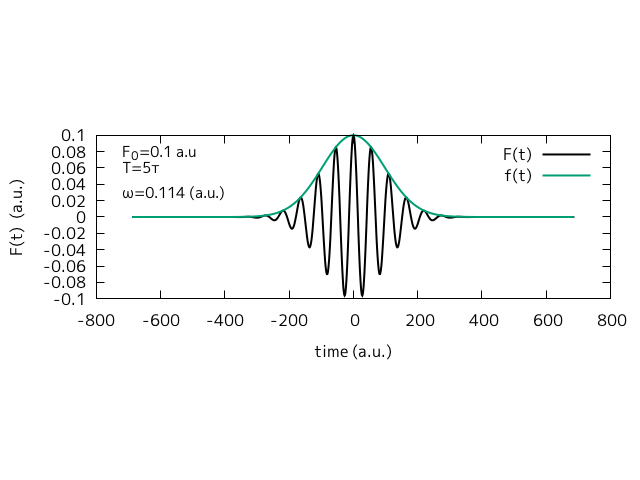
\includegraphics[scale=1., trim={0 20 0 120},clip]{images/field_01_114_5t.png}
%%
%%%%\caption{Eigenvalues.}
%%%\label{fig:pemd_0114}
%% \end{figure}
%%
%%
%%\end{minipage}
%%\end{textblock*}
%%
%%
%%\begin{textblock*}{700pt}(500pt,950pt)
%%\small
%%
%%$I_0 = 3.51 \times 10^{16}\,{\rm W/cm^2} 
%%\longleftrightarrow F_0 = 1\,{\rm a.u.}$ 
%%
%%\end{textblock*}
%%
%%
%%
%%
%%\begin{textblock*}{500pt}(1100pt,850pt)
%% \mbox{\normalsize \textbf{Quantum Field}} \hspace{60pt}
%% \begin{align}
%%&   \boldsymbol{\rm A}
%%  = \sum_\nu \boldsymbol{\rm A}_\nu \left( \hat{a}^{\dagger}_\nu 
%%    + \hat{a}_\nu\right), \nonumber \\
%%& \boldsymbol{F}(t) = -\frac{\partial \boldsymbol{A}(t)}{\partial t} \nonumber \\
%%& \mbox{If}\hspace{20pt} F_0 \gg 0.005\,{\rm a.u.}
%% \longrightarrow \hspace{20pt}\mbox{\textbf{Classical treatment allowed}} \nonumber\\
%%& \hspace{20pt} \boldsymbol{F}(t) = \boldsymbol{F_0}\,e^{-(2t^\prime/\tau)^2} \cos (\omega t^\prime) \nonumber,\hspace{20pt}
%%\hspace{40pt}\mbox{\footnotesize $t^{\prime} = t - T/2, \hspace{20pt} 0 \leqslant t \leqslant T, 
%%\hspace{20pt}\tau = 2\pi n_{\rm oc}/\omega \hspace{20pt}, n_{\rm oc} =5, \hspace{20pt} T = n\tau$ \nonumber}
%% \end{align}
%%
%%\end{textblock*}
%%
%%
%%
%%%\begin{textblock*}{500pt}(1700pt,850pt)
%%%%\centering
%%%%\rotatebox{90}{
%%% \begin{minipage}{0.6\linewidth}
%%% \begin{figure}[tp]
%%% 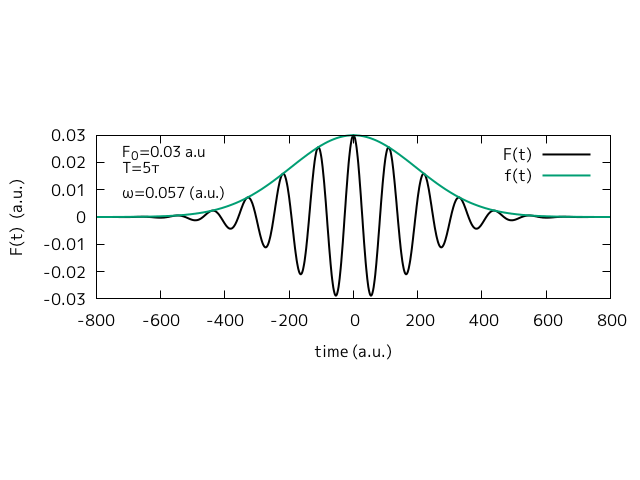
\includegraphics[scale=.8, trim={0 0 0 120},clip]{images/field_003_057_5t.png}
%%%
%%%%%\caption{Eigenvalues.}
%%%%\label{fig:pemd_0114}
%%% \end{figure}
%%%
%%%\end{minipage}
%%%\end{textblock*}
%%
%%
%%
%%
%%\begin{textblock*}{\textwidth}(1100pt,1250pt)
%%{\huge\textbf {4. Results}} \\\vspace{20pt}
%%{\normalsize{\textbf{Dipole moment of the particle \hspace{50pt}$\xrightarrow{\hspace{100pt}} $}}} 
%%\end{textblock*}
%%
%%
%%\begin{textblock*}{700pt}(1800pt,1200pt)
%%%\centering
%%%\rotatebox{90}{
%%%  \small \textbf{Basic strong field phenomena}
%% \begin{minipage}{0.6\linewidth}
%% \begin{figure}[tp]
%% 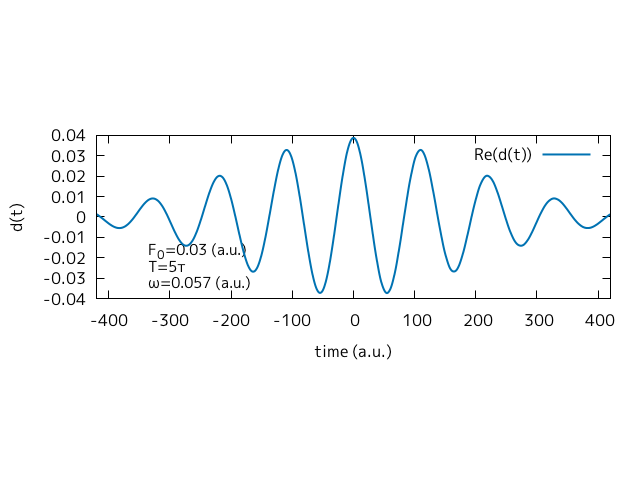
\includegraphics[scale=.8, trim={0 0 20 100},clip]{images/057_f003_d_t.png}
%%
%%%%\caption{Eigenvalues.}
%%%\label{fig:pemd_0114}
%% \end{figure}
%%
%%\end{minipage}
%%\end{textblock*}
%%
%%
%%\begin{textblock*}{700pt}(1800pt,1360pt)
%%%\centering
%%%\rotatebox{90}{
%%%  \small \textbf{Basic strong field phenomena}
%% \begin{minipage}{0.6\linewidth}
%% \begin{figure}[tp]
%% 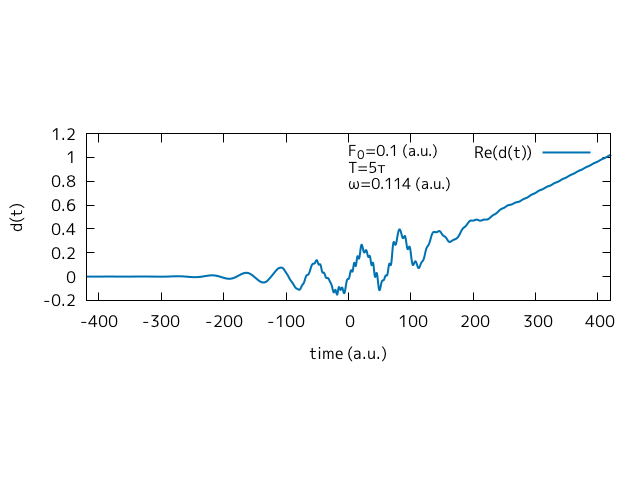
\includegraphics[scale=.8, trim={0 0 20 100},clip]{images/114_f01_d_t.png}
%%
%%%%\caption{Eigenvalues.}
%%%\label{fig:pemd_0114}
%% \end{figure}
%%
%%\end{minipage}
%%\end{textblock*}
%%
%%
%%\begin{textblock*}{0.3\textwidth}(1100pt,1420pt)
%%{\normalsize{\textbf{Photoelectron momentum distribution 
%%and High harmonic generation}\hspace{50pt}$\downarrow$}} 
%%\end{textblock*}
%%
%%\begin{textblock*}{700pt}(1050pt,1520pt)
%%%\centering
%%%\rotatebox{90}{
%%%  \small \textbf{Basic strong field phenomena}
%% \begin{minipage}{0.6\linewidth}
%% \begin{figure}[tp]
%% 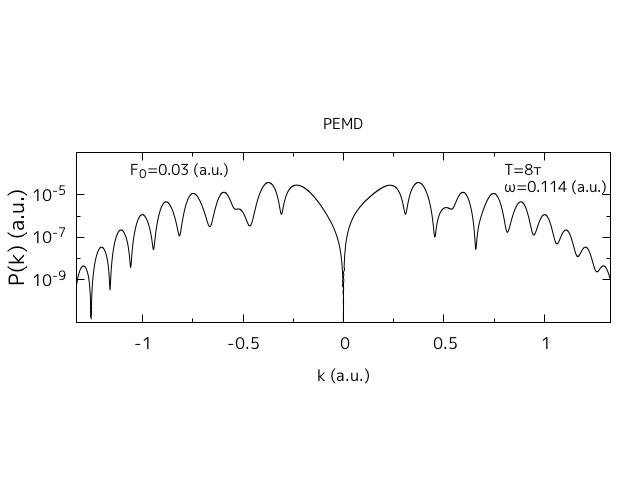
\includegraphics[scale=1., trim={0 0 20 150},clip]{images/114_f003_pemd.png}
%%
%%%%\caption{Eigenvalues.}
%%%\label{fig:pemd_0114}
%% \end{figure}
%%
%%\end{minipage}
%%\end{textblock*}
%%
%%
%%\begin{textblock*}{700pt}(1050pt,1730pt)
%%%\centering
%%%\rotatebox{90}{
%%%  \small \textbf{Basic strong field phenomena}
%% \begin{minipage}{0.6\linewidth}
%% \begin{figure}[tp]
%% 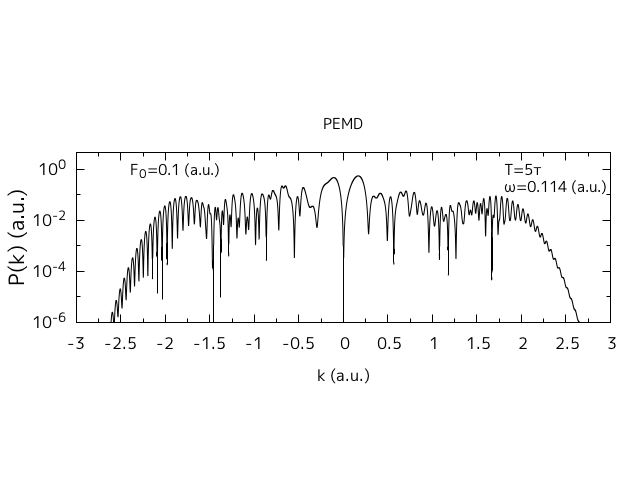
\includegraphics[scale=1., trim={0 0 20 150},clip]{images/114_f01_pemd.png}
%%
%%%%\caption{Eigenvalues.}
%%%\label{fig:pemd_0114}
%% \end{figure}
%%
%%\end{minipage}
%%\end{textblock*}
%%
%%
%%\begin{textblock*}{700pt}(1050pt,1940pt)
%%%\centering
%%%\rotatebox{90}{
%%%  \small \textbf{Basic strong field phenomena}
%% \begin{minipage}{0.6\linewidth}
%% \begin{figure}[tp]
%% 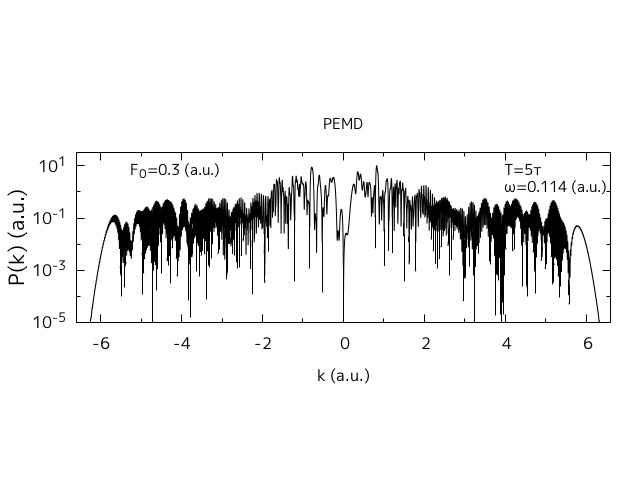
\includegraphics[scale=1., trim={0 0 20 150},clip]{images/114_f03_pemd.png}
%%
%%%%\caption{Eigenvalues.}
%%%\label{fig:pemd_0114}
%% \end{figure}
%%
%%\end{minipage}
%%\end{textblock*}
%%
%%
%%
%%\begin{textblock*}{700pt}(1050pt,2280pt)
%%%\centering
%%%\rotatebox{90}{
%%%  \small \textbf{Basic strong field phenomena}
%% \begin{minipage}{0.6\linewidth}
%% \begin{figure}[tp]
%% 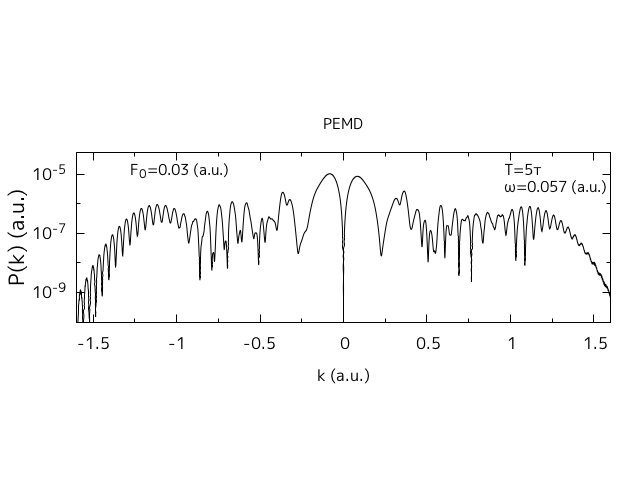
\includegraphics[scale=1., trim={0 0 20 150},clip]{images/057_f003_pemd.png}
%%
%%%%\caption{Eigenvalues.}
%%%\label{fig:pemd_0114}
%% \end{figure}
%%
%%\end{minipage}
%%\end{textblock*}
%%
%%
%%\begin{textblock*}{700pt}(1050pt,2490pt)
%%%\centering
%%%\rotatebox{90}{
%%%  \small \textbf{Basic strong field phenomena}
%% \begin{minipage}{0.6\linewidth}
%% \begin{figure}[tp]
%% 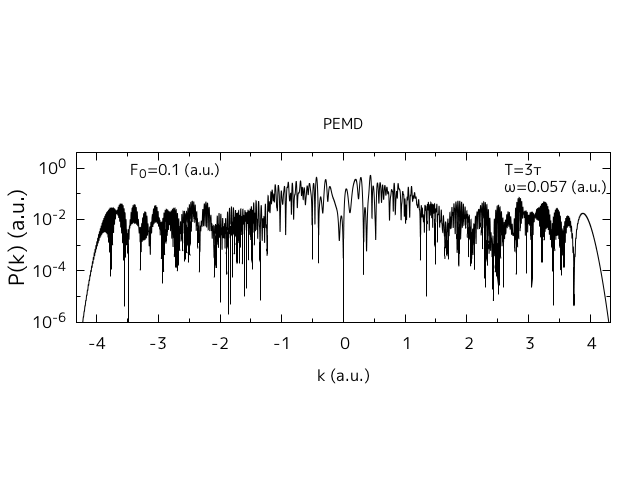
\includegraphics[scale=1., trim={0 0 20 150},clip]{images/057_f01_pemd.png}
%%
%%%%\caption{Eigenvalues.}
%%%\label{fig:pemd_0114}
%% \end{figure}
%%
%%\end{minipage}
%%\end{textblock*}
%%
%%
%%
%%
%%
%%
%%
%%
%%
%%
%%
%%
%%\begin{textblock*}{700pt}(1700pt,1650pt)
%%%\centering
%%%\rotatebox{90}{
%%%  \small \textbf{Basic strong field phenomena}
%% \begin{minipage}{0.6\linewidth}
%% \begin{figure}[tp]
%% 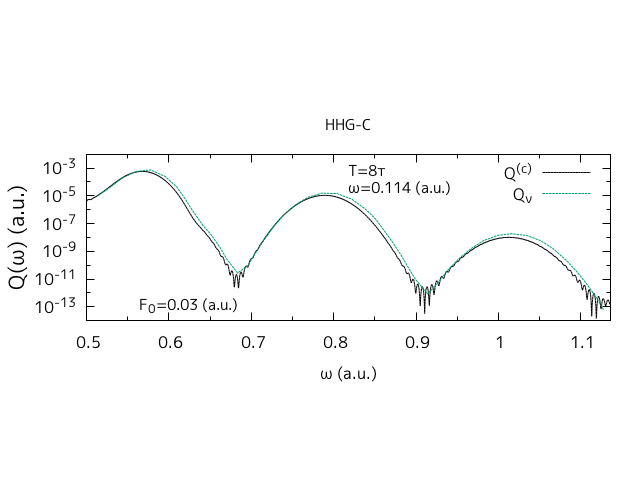
\includegraphics[scale=1., trim={0 0 0 150},clip]{images/114_f003_hhg.png}
%%
%%%%\caption{Eigenvalues.}
%%%\label{fig:pemd_0114}
%% \end{figure}
%%
%%
%%\end{minipage}
%%\end{textblock*}
%%
%%
%%\begin{textblock*}{700pt}(1700pt,1860pt)
%%%\centering
%%%\rotatebox{90}{
%%%  \small \textbf{Basic strong field phenomena}
%% \begin{minipage}{0.6\linewidth}
%% \begin{figure}[tp]
%% 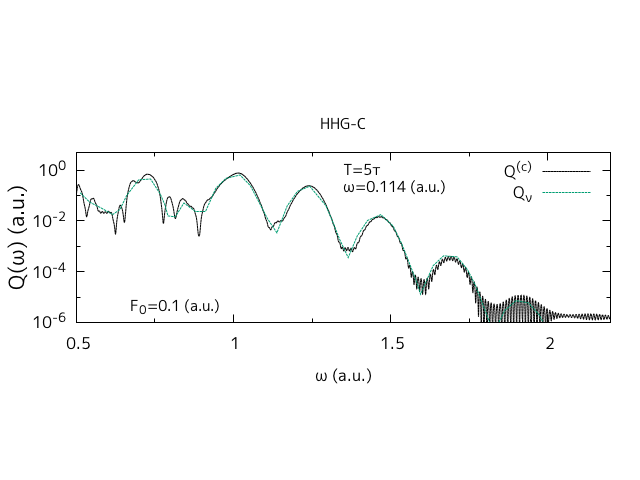
\includegraphics[scale=1., trim={0 0 0 150},clip]{images/114_f01_hhg.png}
%%
%%%%\caption{Eigenvalues.}
%%%\label{fig:pemd_0114}
%% \end{figure}
%%
%%
%%\end{minipage}
%%\end{textblock*}
%%
%%
%%\begin{textblock*}{700pt}(1700pt,2070pt)
%%%\centering
%%%\rotatebox{90}{
%%%  \small \textbf{Basic strong field phenomena}
%% \begin{minipage}{0.6\linewidth}
%% \begin{figure}[tp]
%% 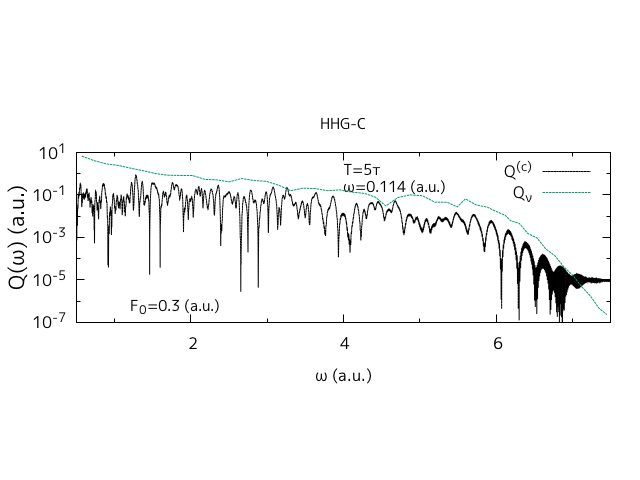
\includegraphics[scale=1., trim={0 0 0 144},clip]{images/114_f03_hhg.png}
%%
%%%%\caption{Eigenvalues.}
%%%\label{fig:pemd_0114}
%% \end{figure}
%%
%%
%%\end{minipage}
%%\end{textblock*}
%%
%%
%%\begin{textblock*}{700pt}(1700pt,2380pt)
%%%\centering
%%%\rotatebox{90}{
%%%  \small \textbf{Basic strong field phenomena}
%% \begin{minipage}{0.6\linewidth}
%% \begin{figure}[tp]
%% 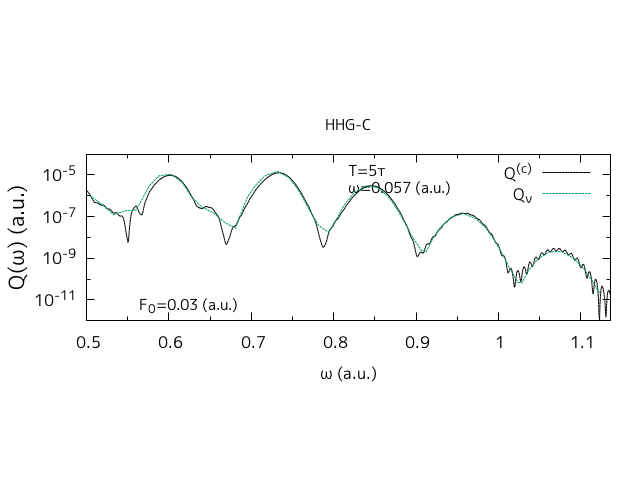
\includegraphics[scale=1., trim={0 0 0 150},clip]{images/057_f003_hhg.png}
%%
%%%%\caption{Eigenvalues.}
%%%\label{fig:pemd_0114}
%% \end{figure}
%%
%%
%%\end{minipage}
%%\end{textblock*}
%%
%%
%%\begin{textblock*}{700pt}(1700pt,2590pt)
%%%\centering
%%%\rotatebox{90}{
%%%  \small \textbf{Basic strong field phenomena}
%% \begin{minipage}{0.6\linewidth}
%% \begin{figure}[tp]
%% 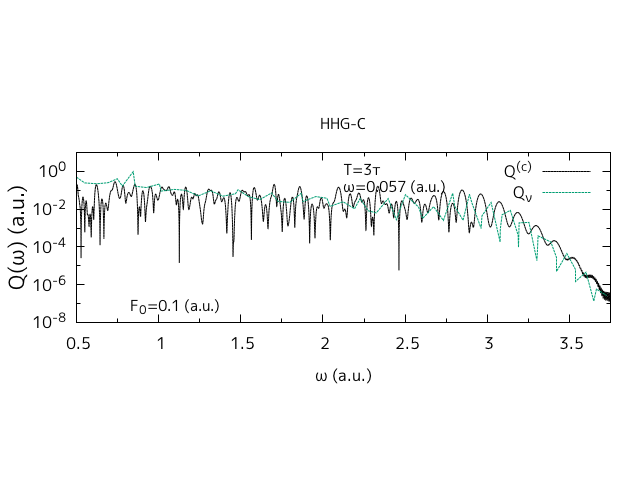
\includegraphics[scale=1., trim={0 0 0 150},clip]{images/057_f01_hhg.png}
%%
%%%%\caption{Eigenvalues.}
%%%\label{fig:pemd_0114}
%% \end{figure}
%%
%%
%%\end{minipage}
%%\end{textblock*}
%%
%%
%%\begin{textblock*}{600pt}(1750pt,2325pt)
%%\scriptsize
%%\centering 
%%\textbf{
%%Quantum correction required for 
%%$\boldsymbol{F_0 \geqslant 0.3\,{\rm a.u.}}$}
%%\end{textblock*}
%%
%%
%%
%%
%%\begin{textblock*}{0.5\textwidth}(1100pt,2850pt)
%%{\huge\textbf {5. Conclusion}} \\\vspace{30pt}
%%\begin{itemize}
%%\small
%%\item The classical ansatz used to evaluate HHG spectra 
%%ceases to be a good approximation for field strengths approaching unity
%%\item Since lasers of intensity greater than 
%%$I_0$ are now available, 
%%a more appropriate theoretical treatment for HHG is highly desirable
%%\vspace{20pt}
%%\item The present study aims at extending this previous result 
%%to realistic  atomic system 
%%\end{itemize}
%%\end{textblock*}
%%
%%
\end{frame}
\end{document}
